\documentclass{beamer}
\usepackage[english, russian, ukrainian]{babel}
\usepackage[utf8]{inputenc}
\graphicspath{{pictures/}}
% Presentation style
\usetheme[numbers]{Singapore}
\usepackage[percent]{overpic}

\setbeamertemplate{navigation symbols}{}

\defbeamertemplate*{footline}{Singapore} {
\hbox{
\begin{beamercolorbox}[wd=.5\paperwidth,ht=2.5ex,dp=1.125ex,leftskip=12.cm,rightskip=.3cm]{author in head/foot}
\insertframenumber{}
\end{beamercolorbox}
}
}

\begin{document}

\title{Задача BE (Луна)}
\author{Олексій Лубинець, Валерія Жовковська 5 курс, ФВЕ}
\institute{\normalsize Об'єктно-орієнтоване програмування}
\date{\today} 

%######## COVER PAGE ####################################################################
\thispagestyle{empty}% removes page number only on the current (title) page
\frame{\titlepage}
%########################################################################################

\begin{frame}{Умова задачі}
На фотографиях ночного неба можно различить только два цвета: черный и белый.
\\
Будем считать, что Луна на снимке выглядит как круг с центром в точке изображения C и целым неотрицательным радиусом r, то есть как множество белых точек, расстояние от центров которых до точки C не больше r. Луна полностью поместилась на снимке.
\\
Также некоторые звезды могут присутствовать на снимке в виде отдельных белых точек. Таких точек, как и звезд на небе, может быть достаточно много.
\\
Напишите программу, которая по изображению найдет наибольший возможный радиус круга, который соответствует Луне.
\end{frame}

\begin{frame}{Приклад}
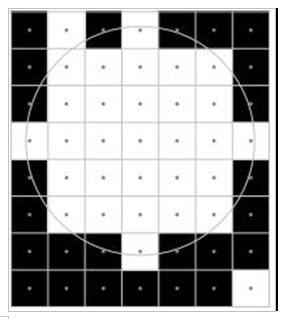
\includegraphics[scale=0.5]{moon.jpg}
\end{frame}

\begin{frame}{Input-Output}
\begin{block}{Input format}
В первой строке ввода записаны целые числа w и h — горизонтальное и вертикальное разрешение снимка, соответственно (1 <= w, h <= 200). В следующих h строках записано по w символов "." (черная точка) или "*" (белая точка).
\end{block}
\begin{block}{Output format}
В одной строке выведите натуральное число — максимальный радиус изображения Луны. Гарантируется, что корректный ответ существует.
\end{block}
\end{frame}

\begin{frame}{''Критерій Місяця Метод No.1''}
Спосіб гарантувати, що ми знайшли Місяць радіуса R з центром C - перевірити всі пікселі, відстань до яких не перевищує R, чи є вони білими.
\\
Тож пробігаємо всі пікселі, крім ``рамочки`` на предмет того, чи можуть вони бути центром Місяця і якщо можуть, то якого радіуса. Максимальний із знайдених радіусів і буде відповіддю на задачу.
\end{frame}

\begin{frame}{Визначення радіуса для Місяця з центром у конкретному пікселі}
Заздалегідь для кожного ``потенційного радіуса`` визначаються точки (а саме зсуви по X та Y), які будуть для Місяця з таким радіусом граничними.
\\
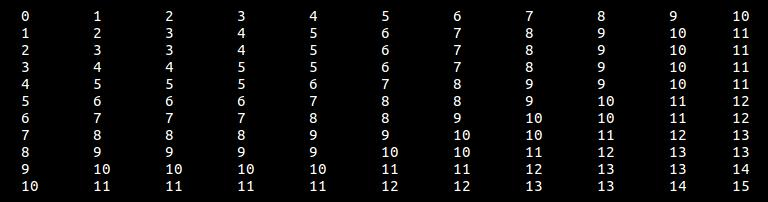
\includegraphics[scale=0.4]{maxrad.jpg}
\end{frame}

\begin{frame}{Визначення радіуса для Місяця з центром у конкретному пікселі}
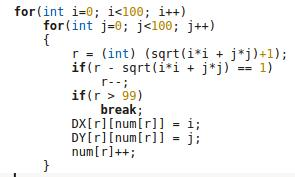
\includegraphics[scale=0.5]{maxradcode.jpg}
\end{frame}

\begin{frame}{Пошук по всім пікселям}
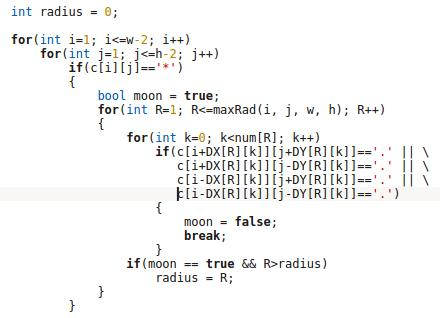
\includegraphics[scale=0.5]{runallpixels.jpg}
\end{frame}

\begin{frame}{``Критерій Місяця Метод No.2``}
Спосіб гарантувати, що ми знайшли Місяць радіуса R з центром C - для кожного пікселя знайти відстань до найближчого чорного пікселя. Піксель, найбільш віддалений від чорних, буде центром кола C. Відстань від краю до визначеного пікселя буде відповідати радіусу кола R. 
\\
Тож пробігаємо всі пікселі, крім ``рамочки``, визначаючи кількість білих сусідів по вертикалі та горизонталі. 

\end{frame}

\begin{frame}
На першому кроці для білої клітинки відстань до найближчої чорної клітинки -- \textbf{1}, для чорної -- \textbf{0} \\
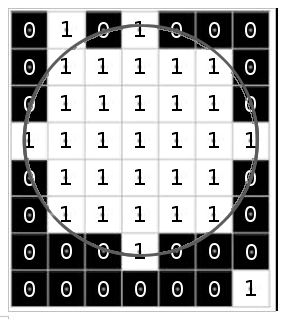
\includegraphics[scale=0.5]{moon_1.jpg}

\end{frame}

\begin{frame}
Виконується чотири проходи:  \\

\begin{figure}[h]
  \centering  
  \begin{overpic}[scale=0.30]{moon_1.jpg}
     \put(-5,102){\huge{$\Rightarrow$}}  
     \put(-15,90){\huge{$\Downarrow$}}  
  \end{overpic}
%  \hfill
  \begin{overpic}[scale=0.30]{moon_1.jpg}
     \put(78,102){\huge{$\Leftarrow$}}  
     \put(95,90){\huge{$\Downarrow$}}  
  \end{overpic}

  \begin{overpic}[scale=0.30]{moon_1.jpg}
     \put(-5,-12){\huge{$\Rightarrow$}}  
     \put(-15,0){\huge{$\Uparrow$}}  
  \end{overpic}
%  \hfill
  \begin{overpic}[scale=0.30]{moon_1.jpg}
     \put(78,-12){\huge{$\Leftarrow$}}  
     \put(95,0){\huge{$\Uparrow$}}  
  \end{overpic}

%\center{\includegraphics[width=0.5\linewidth]{pictures/TzEtac_newBkg.png}}
%\caption{Simultaneous $\chi^2$ integral fit to $\eta_c$ (left) and $J/\psi$ (right) $t_z$ distributions. The yield value and its uncertainty in each bin are obtained from the fit of invariant mass $M(p\bar{p})$}
%\label{pic:tzTot}
\end{figure}

\end{frame}


\begin{frame}
Значення у клітинці відповідає \textbf{мінімальному} зі значень у сусідніх \textbf{пройдених} клітинках. Фінальне значення - мінімальне з усіх матриць.
\begin{columns}
\begin{column}{0.7\textwidth}
\begin{figure}[h]
  \centering  
  \begin{overpic}[scale=0.40]{Up.png}
     \put(-35,102){\huge{$\Rightarrow$}}  
     \put(-45,90){\huge{$\Downarrow$}}  
  \end{overpic}
%  \hfill
  \begin{overpic}[scale=0.40]{Left.png}
     \put(78,102){\huge{$\Leftarrow$}}  
     \put(95,90){\huge{$\Downarrow$}}  
  \end{overpic}

  \begin{overpic}[scale=0.40]{Right.png}
     \put(-35,-12){\huge{$\Rightarrow$}}  
     \put(-45,0){\huge{$\Uparrow$}}  
  \end{overpic}
%  \hfill
  \begin{overpic}[scale=0.40]{Down.png}
     \put(78,-12){\huge{$\Leftarrow$}}  
     \put(95,0){\huge{$\Uparrow$}}  
  \end{overpic}
\end{figure}

\end{column}
\begin{column}{0.3\textwidth}
\begin{figure}[h]
  \centering  
  \begin{overpic}[scale=0.40]{Final.png}
     \put(-50,42){\huge{$\rightrightarrows$}}  
  \end{overpic}
\end{figure}
\end{column}

\end{columns}


\end{frame}


\begin{frame}{Визначення стартових матриць}
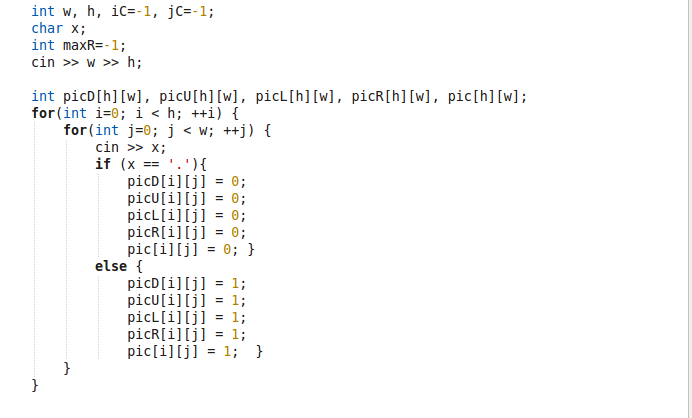
\includegraphics[scale=0.4]{Read.png}
\end{frame}

\begin{frame}{Визначення радіуса для Місяця з центром для певного напрямку руху по матриці}
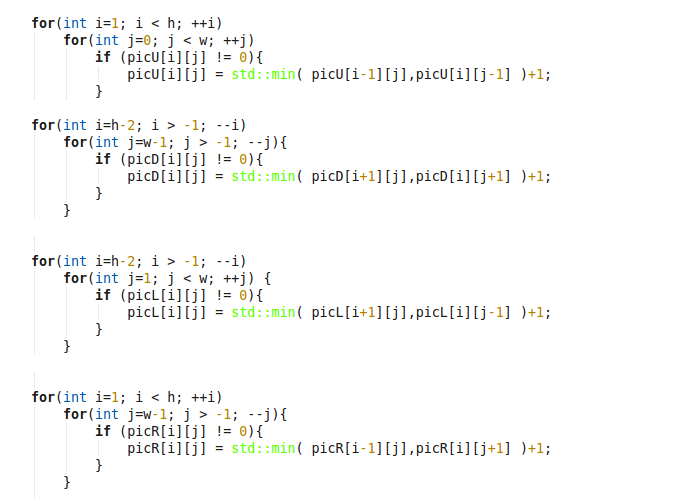
\includegraphics[scale=0.4]{MinimumLocal.png}
\end{frame}

\begin{frame}{Визначення радіуса для Місяця}
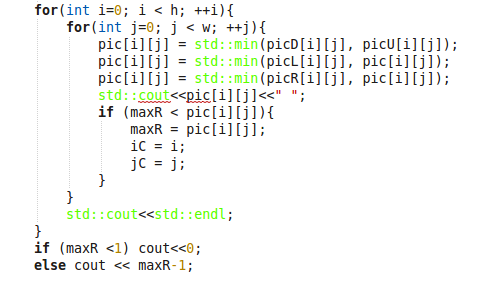
\includegraphics[scale=0.5]{MinimumGlobal.png}
\end{frame}


\end{document}
